\documentclass[]{article}
\usepackage{lmodern}
\usepackage{amssymb,amsmath}
\usepackage{ifxetex,ifluatex}
\usepackage{fixltx2e} % provides \textsubscript
\ifnum 0\ifxetex 1\fi\ifluatex 1\fi=0 % if pdftex
  \usepackage[T1]{fontenc}
  \usepackage[utf8]{inputenc}
\else % if luatex or xelatex
  \ifxetex
    \usepackage{mathspec}
  \else
    \usepackage{fontspec}
  \fi
  \defaultfontfeatures{Ligatures=TeX,Scale=MatchLowercase}
\fi
% use upquote if available, for straight quotes in verbatim environments
\IfFileExists{upquote.sty}{\usepackage{upquote}}{}
% use microtype if available
\IfFileExists{microtype.sty}{%
\usepackage{microtype}
\UseMicrotypeSet[protrusion]{basicmath} % disable protrusion for tt fonts
}{}
\usepackage[margin=1in]{geometry}
\usepackage{hyperref}
\hypersetup{unicode=true,
            pdftitle={Food Balance Sheet workflow in the Statistical Working System},
            pdfauthor={Cristina Muschitiello Food and Agriculture Organization of the United Nations},
            pdfborder={0 0 0},
            breaklinks=true}
\urlstyle{same}  % don't use monospace font for urls
\usepackage{graphicx,grffile}
\makeatletter
\def\maxwidth{\ifdim\Gin@nat@width>\linewidth\linewidth\else\Gin@nat@width\fi}
\def\maxheight{\ifdim\Gin@nat@height>\textheight\textheight\else\Gin@nat@height\fi}
\makeatother
% Scale images if necessary, so that they will not overflow the page
% margins by default, and it is still possible to overwrite the defaults
% using explicit options in \includegraphics[width, height, ...]{}
\setkeys{Gin}{width=\maxwidth,height=\maxheight,keepaspectratio}
\IfFileExists{parskip.sty}{%
\usepackage{parskip}
}{% else
\setlength{\parindent}{0pt}
\setlength{\parskip}{6pt plus 2pt minus 1pt}
}
\setlength{\emergencystretch}{3em}  % prevent overfull lines
\providecommand{\tightlist}{%
  \setlength{\itemsep}{0pt}\setlength{\parskip}{0pt}}
\setcounter{secnumdepth}{5}
% Redefines (sub)paragraphs to behave more like sections
\ifx\paragraph\undefined\else
\let\oldparagraph\paragraph
\renewcommand{\paragraph}[1]{\oldparagraph{#1}\mbox{}}
\fi
\ifx\subparagraph\undefined\else
\let\oldsubparagraph\subparagraph
\renewcommand{\subparagraph}[1]{\oldsubparagraph{#1}\mbox{}}
\fi

%%% Use protect on footnotes to avoid problems with footnotes in titles
\let\rmarkdownfootnote\footnote%
\def\footnote{\protect\rmarkdownfootnote}

%%% Change title format to be more compact
\usepackage{titling}

% Create subtitle command for use in maketitle
\newcommand{\subtitle}[1]{
  \posttitle{
    \begin{center}\large#1\end{center}
    }
}

\setlength{\droptitle}{-2em}
  \title{Food Balance Sheet workflow\\
in the Statistical Working System}
  \pretitle{\vspace{\droptitle}\centering\huge}
  \posttitle{\par}
  \author{Cristina Muschitiello\\
Food and Agriculture Organization of the United Nations}
  \preauthor{\centering\large\emph}
  \postauthor{\par}
  \predate{\centering\large\emph}
  \postdate{\par}
  \date{24 May 2018}

\usepackage{lscape}
\usepackage{booktabs}
\usepackage{longtable}
\usepackage{array}
\usepackage{multirow}
\usepackage[table]{xcolor}
\usepackage{wrapfig}
\usepackage{float}
\usepackage{colortbl}
\usepackage{pdflscape}
\usepackage{tabu}
\usepackage{threeparttable}
\usepackage{threeparttablex}
\usepackage[normalem]{ulem}
\usepackage{makecell}

\usepackage{draftwatermark}
\usepackage{makeidx}
\makeindex
\usepackage{float}
\floatplacement{figure}{H}
\usepackage{amsmath}
\usepackage{amssymb}
\usepackage{amsthm}
\usepackage{mathtools}

\begin{document}
\maketitle
\begin{abstract}
This vignette provides a description of the workflow and dependencies of
operations in the Statistical Working System for the production of Food
Balance Sheets.
\end{abstract}

{
\setcounter{tocdepth}{4}
\tableofcontents
}
\newpage

\listoftables

\listoffigures

\newpage

\subsection*{Disclaimer}\label{disclaimer}
\addcontentsline{toc}{subsection}{Disclaimer}

This Working Paper should not be reported as representing the official
view of the FAO. The views expressed in this Working Paper are those of
the author and do not necessarily represent those of the FAO or FAO
policy. Working Papers describe research in progress by the authors and
are published to elicit comments and to further discussion.

This paper is dynamically generated on \today{} and is subject to
changes and updates.

\section*{The Overall Workflow of The
FBS}\label{the-overall-workflow-of-the-fbs}
\addcontentsline{toc}{section}{The Overall Workflow of The FBS}

The process of creating FBSs starts by collecting all data for the
different variables of the Food Balance Sheet Framework\footnote{For
  definitions and an extended description of the motivation behind the
  development of FBS, see FAO, 2001, \emph{Food Balance Sheets: A
  Handbook}, available at:
  \url{http://www.fao.org/docrep/003/X9892E/X9892E00.HTM}. Accessed on
  19 January 2017. Moreover see \emph{Standardization \& Balancing for
  Food Balance Sheet Calculation}, in the \emph{Standardization \&
  Balancing} module's documentation on
  \href{https://github.com/SWS-Methodology/faoswsStandardization/tree/master/documentation}{\emph{GitHub}}}.
The data of each variable are generally checked and imputed in time
series. The set of operations required for creating/checking time series
of data for each variable is called \emph{module}. A
\textbf{\emph{module}}, in the FBS Framework, is an R-script, written by
an R-developer and integrate inside the \textbf{\emph{Statistical
Working System (SWS)}}\footnote{SWS is an internal Working System
  providing a platform for statisticians and statistical clers to
  collect, collate, validate and correct data. Moreover, the platfors
  supports the possibility of performing imputations of data based on
  statisticians' knowledge and development.} by means of \emph{plugins}.
There is at least one module (there might be more) for each variable of
the FBS. Each module produces figures that are collected in a dataset
inside the SWS for future uses or publication. Output data of a module
may become input data of another module, this circumstance creating a
precise sequence for the execution of a complete FBS.

\section*{Definitions}\label{definitions}
\addcontentsline{toc}{section}{Definitions}

\section*{B. Standardization and
Balancing}\label{b.-standardization-and-balancing}
\addcontentsline{toc}{section}{B. Standardization and Balancing}

\section{The Overall Workflow}\label{the-overall-workflow}

The \emph{Standardiation \& Balancing} process is presented in Figure
\ref{fig:f9}. It involves 5 main steps and requires a some auxiliary
information table.

The 5 steps are:

\begin{enumerate}
\def\labelenumi{\arabic{enumi}.}
\tightlist
\item
  Data Pull,
\item
  Sua Filling,
\item
  Standardization,
\item
  Balancing,
\item
  FBS aggregation.
\end{enumerate}

The additional information's tables are:

\begin{itemize}
\tightlist
\item
  \emph{Utilization Table},
\item
  \emph{Zero-Weight} table,
\item
  \emph{cut} table,
\item
  \emph{Fbs Tree}.
\end{itemize}

All the steps and the table will be described across the present
document, after having introduced the the basic equation of FBS and the
\emph{Commodity tree} which represents the structure of the set of
commodity involved in the Food Balance Sheets.

\begin{figure}[H]

{\centering 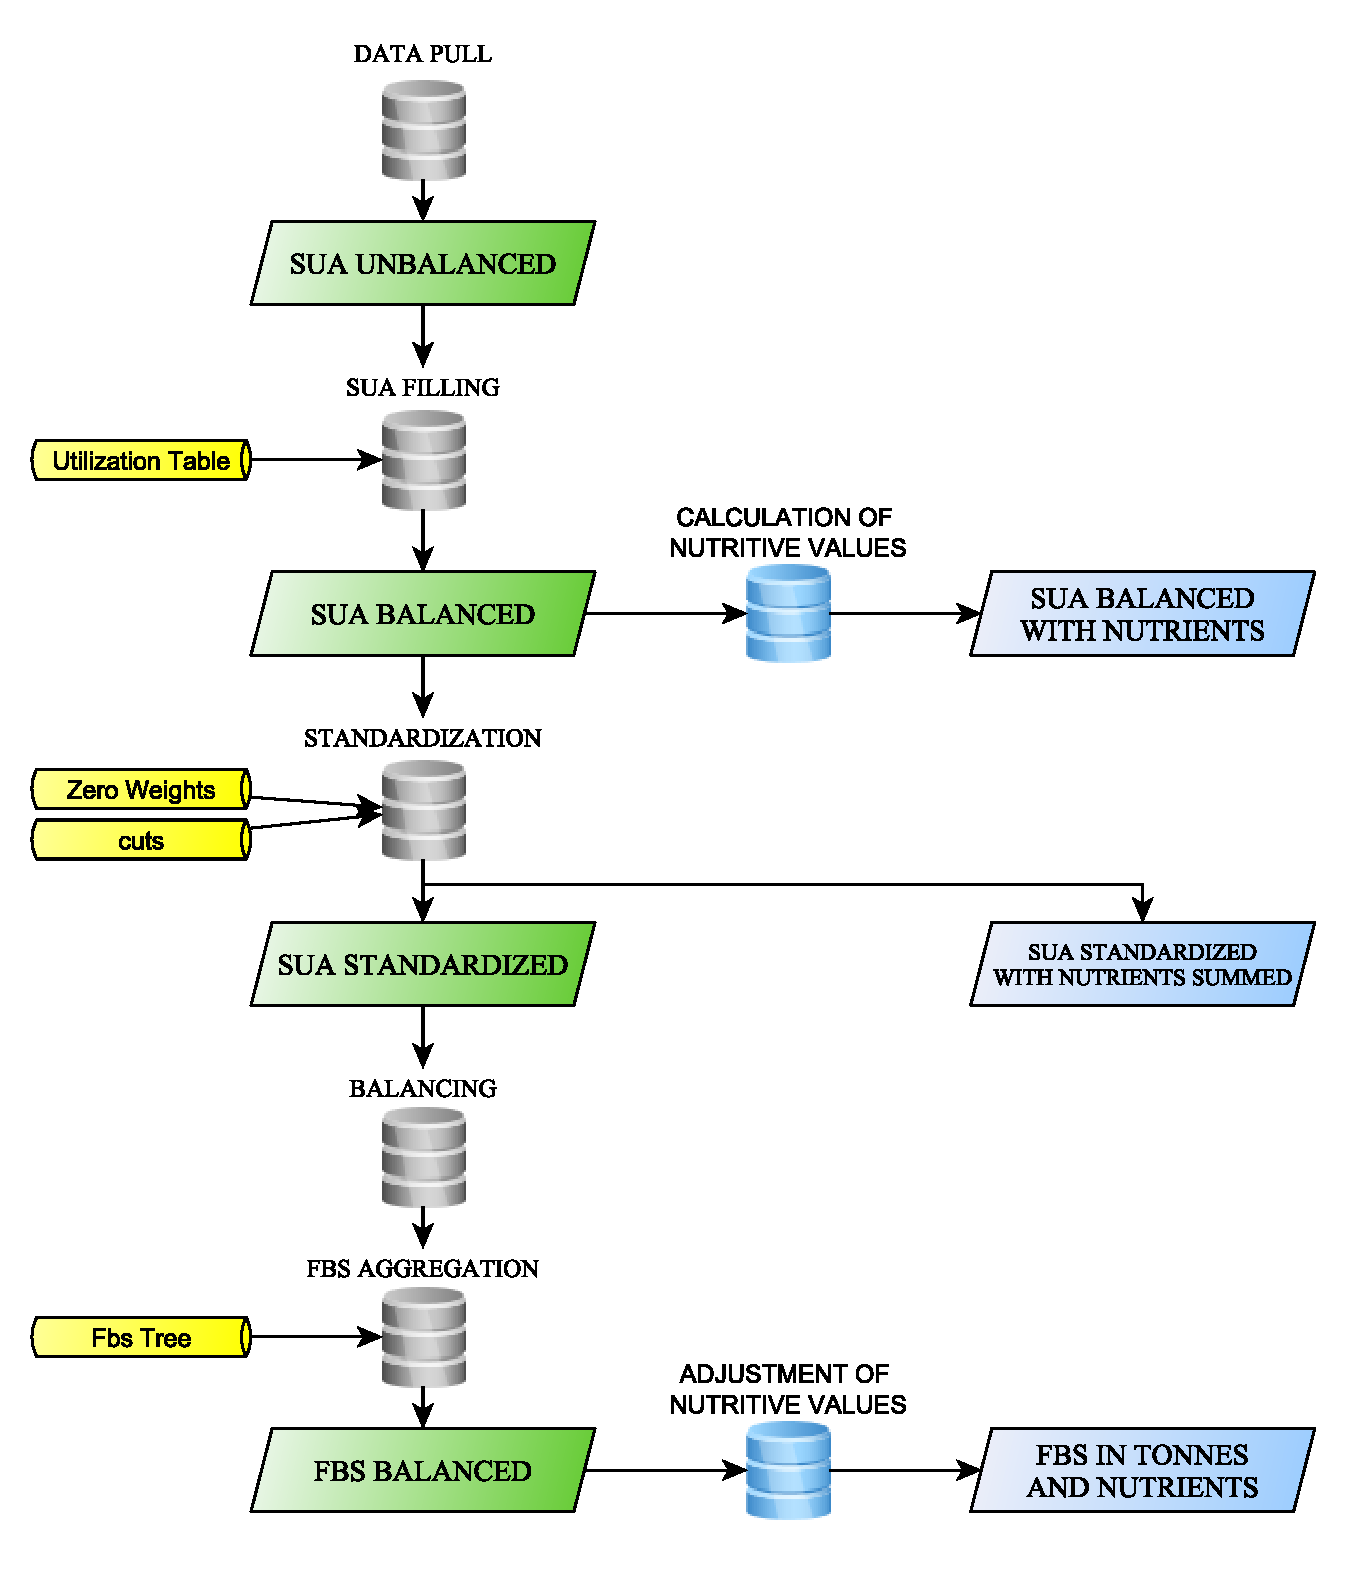
\includegraphics[width=0.8\linewidth]{images/09_overall} 

}

\caption{\label{fig:f9}Standardization and Balancing Overall Workflow}\label{fig:f9}
\end{figure}

\section*{Commodity Tree}\label{commodity-tree}
\addcontentsline{toc}{section}{Commodity Tree}

The process of combining commodity balances for creating Food Balance
Sheets is based on a structured and clear set of relationships between
commodity given by the \emph{Commodity tree}. The majority of the
commodities are produced from one (or more) commodity (/ies), called
\emph{parent} commodity(/ies), and/or are themselfes parent of one (or
more) \emph{child} (\emph{children}) commodity (/ies). These structure
creates an intense and articulated network of relationships at different
levels: primary commodities, like crops, are \emph{parent} commodities
and, also, \emph{zero-level} commodities from which \emph{children}
commodities of \emph{level-1} are produced, which are in turn, used to
produce other commodities of a gradually \emph{``lower''} level. In
commodtity trees, the bigger the level number, the lower the processing
level. There are as many commodity trees as the number of process chains
in a country. Fundamental characteristics of commodity trees
are\footnote{For a more detailed description of commodity trees, please
  see the specific documentation. The reference document, at the moment
  is the \emph{tecnical conversion factor} document available in the
  documentation folder on
  \href{https://github.com/SWS-Methodology/faoswsStandardization/tree/master/documentation}{\emph{GitHub}}}:

\begin{enumerate}
\def\labelenumi{\arabic{enumi}.}
\tightlist
\item
  Each commodity tree is represented as a flowchart of the kind
  presented in Figure \ref{fig:f2} where:

  \begin{itemize}
  \tightlist
  \item
    \textbf{\emph{nodes}} represent commodities,
  \item
    \textbf{\emph{edges}} represent production processes ,
  \item
    \textbf{\emph{joints}} indicate where a single production process
    creates more that one commodity. These commodities are, then, called
    \emph{by-products} or \emph{co-products}.
  \end{itemize}
\end{enumerate}

\begin{figure}[H]

{\centering 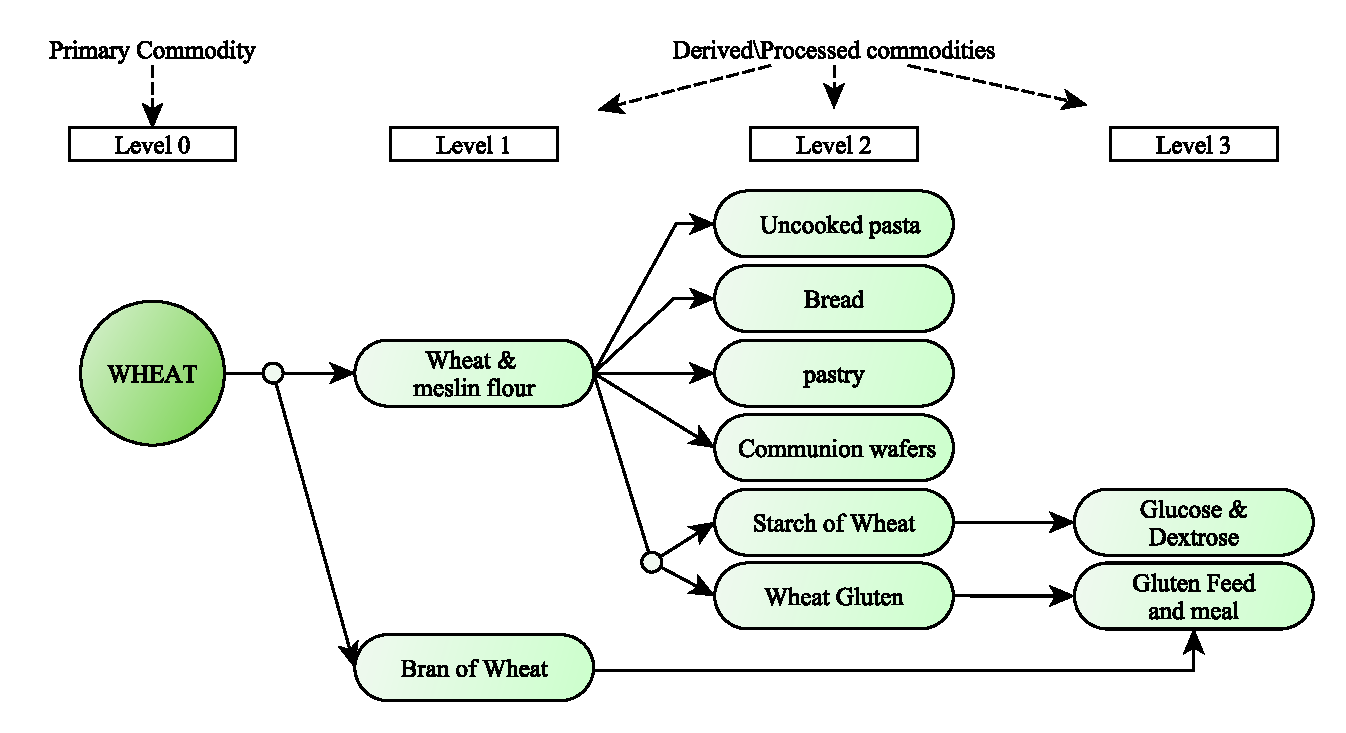
\includegraphics{images/02_WheatTree} 

}

\caption{\label{fig:f2}Commodity Tree for Wheat in China mainland 2014}\label{fig:f2}
\end{figure}

\begin{enumerate}
\def\labelenumi{\arabic{enumi}.}
\setcounter{enumi}{1}
\item
  Not all the countries have the same production processes, because
  countries have different technologies and primary products
  availabilities. Therefore, the commodity trees are not the same across
  countries.
\item
  if a production process is active in a country, this is expressed
  throught the existence of a conversion factor called
  \textbf{\emph{extraction Rate}}. An Extraction rate (\(eR\))
  represents how much amount of the child commodity is produced from 1
  unit of parent commodity. It is expressed as a ratio of the processed
  product obtained from the processing of the parent/originating
  product.
\item
  Some child commodities can be produced starting from more that one
  parent commodity. A second conversion factor exists representing the
  amount of a child commodity that is produced from each parent
  commodity. This conversion factor is called \textbf{\emph{Share}}.
  Shares represent the amount of the child commodity that is produced
  from the specified parent and are expressed as a ratio. Shares are
  generically defined as:
\end{enumerate}

\begin{quote}
\begin{equation}
\label{eq:sharesGen}
s_{cp} = \frac{availability_{p(c)}}{\sum \limits_{p=1}^A{availability_{p(c)}}}
\end{equation}
\end{quote}

\begin{quote}
where \(availability_{p(c)}\) is the availability of each parent \(p\)
of child \(c\) expressed in terms of \(c\) (in \emph{child equivalent}).
\end{quote}

Commodity trees are presented in tables like Table 10, which represents
the same example of Figure \ref{fig:f2}. In the table each production
process is represented in a separate row.

There are some concepts linked to the \emph{Commodity tree} framework:

\begin{itemize}
\tightlist
\item
  \textbf{\emph{Proxy-Primary}} commodities. These are a set of
  commodities that are children of other commodities but, because they
  are important in representing the food availability of a country, are
  not aggregated to their primary commodities, but are kept separated.
  These commodities are \emph{cut} from the tree of the primary
  commodity/ies and, if they can be processed in other products, have
  their own commodity tree. The name \emph{proxy-primary} is assigned
  because they are considered as primary-commodities in the
  \emph{Standardization \& Balancing} process.
\item
  \textbf{\emph{No-Tree}} commodities. These are \emph{zero-level}
  commodities that are primary commodities and are never processed in
  other products. As they are not involved in any production process,
  there is no tree associated to them. Notice that, even a commodity
  that is included in the commodity tree of one Country, might be a
  No-tree commodity for another country or another year, if no
  production processes have been activated for that specific Country or
  year.
\end{itemize}

\section{Data Pull}\label{data-pull}

The process of creating FBSs starts by considering the initial commodity
balance for each CPC commodity, either primary and derived, with the
different variables of the equation (as listed and briefly described in
the previous section) filled with figures as available from official or
other sources and from imputation and estimation methods, when applied.
In other words, the process starts by pulling figures inside a so-called
\emph{Sua Unbalanced}. In this initial account, food processing and ROU
figures are not available (because they, by default, will be measured
during the process), whereas the figures for all other variables have
been already collected, imputed and estimated through a specific
\emph{module} (Figure \ref{fig:f1}).

A \textbf{\emph{module}}, in the FBS Framework, is an R-script, written
by an R-developer, for the execution of a set of operations (either data
import, manipulation, imputation or estimation) required for compiling
the time series of one variable. There is at least one module (there
might be more) for each variable of the FBS. Each module produces
figures that are collected in a dataset inside the
\textbf{\emph{Statistical Working System (SWS)}}\footnote{SWS is an
  internal Working System providing a platform for statisticians and
  statistical clers to collect, collate, validate and correct data.
  Moreover, the platfors supports the possibility of performing
  imputations of data based on statisticians' knowledge and development.}.Output
data of a module may become input data of another module, this
circumstance creating a precise sequence for the execution of a complete
FBS. In the present document, we are analyzing the workflow of the
Standardization process as starts after all the modules have run and
have produced reliable data or each variable. The detailed description
of the workflow for the execution of all the modules of the FBS will be
given in a separate document.\footnote{{[}report the document when it
  will be available{]}}.

\begin{figure}[htbp]
\centering
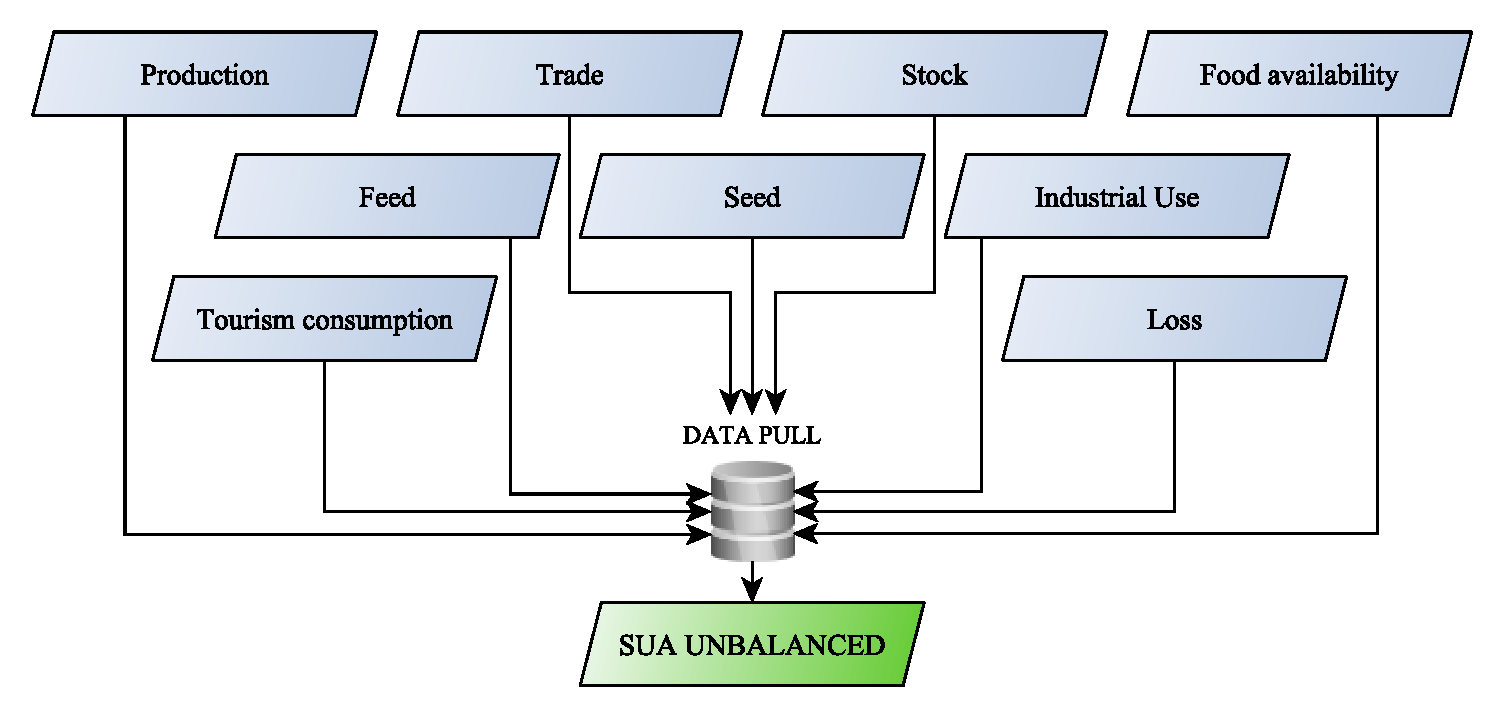
\includegraphics{images/01_pulldata.pdf}
\caption{\label{fig:f1}Data Pull from datasets containing data for each
separate variable}
\end{figure}

\subsection*{the Initial Sua
Unbalanced}\label{the-initial-sua-unbalanced}
\addcontentsline{toc}{subsection}{the Initial Sua Unbalanced}

After pulling all data, the process of compiling Food Balance Sheets is
a non-complete supply-utilization account. The non-completeness of the
SUAs is due to different reasons: first, as already said, some variables
are not collected, nor estimated before the process begins, second there
is the model for industrial use that does not impute or estimate data,
but just collects data from different sources, this opening the strong
possibility not to have values where they are supposed to exist and,
also, not guaranteeing consistency of data over time. Thirdly, modules
might, sometimes, fail in the imputation, because of the strong
complexity and structural diversity of the input data.

\begin{landscape}\begin{table}

\caption{\label{tab:t1}Unbalanced Sua table - China/Wheat/2014 example}
\centering
\resizebox{\linewidth}{!}{\fontsize{18}{20}\selectfont
\begin{tabular}[t]{>{\raggedleft\arraybackslash}p{12em}|>{\raggedright\arraybackslash}p{6em}|>{\raggedright\arraybackslash}p{6em}|>{\raggedright\arraybackslash}p{6em}|>{\raggedright\arraybackslash}p{6em}|>{\raggedright\arraybackslash}p{6em}|>{\raggedright\arraybackslash}p{6em}|>{\raggedright\arraybackslash}p{6em}|>{\raggedright\arraybackslash}p{6em}|>{\raggedright\arraybackslash}p{6em}|>{\raggedright\arraybackslash}p{6em}|>{\raggedright\arraybackslash}p{6em}|>{\raggedright\arraybackslash}p{6em}}
\hline
\multicolumn{1}{r}{\textbf{itemName}} & \multicolumn{1}{c}{\textbf{P}} & \multicolumn{1}{c}{\textbf{I}} & \multicolumn{1}{c}{\textbf{X}} & \multicolumn{1}{c}{\textbf{DSt}} & \multicolumn{1}{c}{\textbf{Fo}} & \multicolumn{1}{c}{\textbf{FP}} & \multicolumn{1}{c}{\textbf{Fe}} & \multicolumn{1}{c}{\textbf{Se}} & \multicolumn{1}{c}{\textbf{T}} & \multicolumn{1}{c}{\textbf{IU}} & \multicolumn{1}{c}{\textbf{L}} & \multicolumn{1}{c}{\textbf{ROU}}\\
\hline
\em{Wheat} & \em{126,208,400} & \em{2,971,249} & \em{957} & \em{1,120,565} & \em{} & \em{-} & \em{29,181,617} & \em{4,277,567} & \em{} & \em{2,985,279} & \em{2,713,000} & \em{-}\\
\hline
Wheat and meslin flo & 70,500,000 & 33,055 & 188,674 &  & 67,300,000 & - &  &  & -17,345 &  &  & -\\
\hline
Mixes and doughs for &  & 6,497 & 38,072 &  & 0 & - & 0 &  & 0 &  &  & -\\
\hline
Other Fructose and S & 126,277 & 3,659 & 162,324 &  & 0 & - &  &  & 0 &  &  & -\\
\hline
Starch of Wheat & 239,816 & 11,035 & 40,311 &  &  & - & 172,196 &  &  & 7,919 &  & -\\
\hline
Wheat Gluten & 25,580 & 877 & 117,373 &  &  & - & 0 &  &  &  &  & -\\
\hline
Communion wafers & 13,263 & 8,796 & 5,822 &  & 16,241 & - &  &  & -4 &  &  & -\\
\hline
Uncooked pasta & 1,415,692 & 12,520 & 22,550 &  & 1,405,661 & - &  &  & -362 &  &  & -\\
\hline
Food Preparations of &  & 69,686 & 21,977 &  & 47,709 & - &  &  & -12 &  &  & -\\
\hline
Bran of Wheat & 21,414,279 & 156,359 & 2,200 &  & 16,500,000 & - & 4,827,244 &  & -4,252 &  &  & -\\
\hline
Gluten Feed and Meal & 793,740 & 160,231 & 529,333 &  &  & - &  &  &  &  &  & -\\
\hline
bread & 15,485 & 2,897 & 4,210 &  & 14,175 & - &  &  & -3 &  &  & -\\
\hline
pastry & 193,950 & 89,593 & 117,630 &  & 165,914 & - &  &  & -43 &  &  & -\\
\hline
\multicolumn{13}{l}{\textsuperscript{a} P=Production, I=Import, X=Export, DSt=Delta Stock, Fo=Food Availability, FP=FoodProcessing, Fe=Feed, Se=Seed, T=Tourism Consumption,}\\
\multicolumn{13}{l}{IU=IndustrialUse, L=Loss, ROU=Residual and other uses}\\
\end{tabular}}
\end{table}
\end{landscape}

S


\end{document}
